\paragraph{}Da bi bila aplikacija "cim bolj prijazna uporabniku je "sla "cez veliko razli"cic in popravkov. V nadaljevanju je opisano kako deluje trenutno najnovej"sa razli"cica 3.0. Izvorna koda je dostopna na spletnem portalu GitHub na naslovu \url{https://github.com/GimVic-app/gimvic-ios}.

\subsection{Struktura}
\paragraph{}
Aplikacija je sestavljena iz dveh delov. Prvi del se ukvarja s pridobivanjem podatkov iz stre"znika, drug del pa se ukvarja s predstavitvijo podatkov uporabniku. Del aplikacije, ki se ukvarja s pridobivanjem in shranjevanjem podatkov je narejen kot knji"znica (Framework), ki jo aplikacija uporablja. S tem lahko kasneje dodam "se druge na"cine prikazovanja urnika uporoabniku (na primer gradnik \textit{ang. widget}), brez da bi ponovno pisal pridobivanje podatkov.

\subsection{Podatki} 
\paragraph{}Podatki, ki jih aplikacija potrebuje, so servirani iz razli"cnih stre"znikov v razli"cnih oblikah zapisa. Urnik je na voljo v JavaScript Array\cite{js-array} obliki, nadome"s"canja pa v JSON\cite{json-wiki}. Jedilnik za "solsko malico in kosilo se nalo"zi na stre"znik v csv\cite{csv-wiki} obliki. Odlo"cil sem se, da bo za podatke skrbel poseben stre"znik, ki bo vse od zgoraj na"stetega zdru"zil v enovito JSON obliko, ker bo tako prikazovanje na telefonu hitrej"se in bolj u"cinkovito. Stre"znik si podatke shranjuje v MySQL\cite{mysql-wiki} podatkovno bazo\cite{rin} in jih nato servira v JSON obliki.

\paragraph{}Pri dostopu do podatkov stre"zniku z URL parametri\cite{query-string-wiki} poda"s ali "zeli"s podatke za profesorja, ali pa za dijaka. Pri profesorju stre"zniku kot parameter poda"s ime profesorja, pri dijaku pa razred in izbirne ozroma maturitetne predmete. Stre"znik nato vrne seznam, kjer vsak element v tem seznamu predstavlaj podatke za dolo"cen dan v tednu. Vsak dan je predstavljen z seznamom v katerem vsak element predstavlja uro.

\begin{figure}[!h]
	\centering
	Primer URL-ja:
	\texttt{http://gimvicapp.404.si/data?addSubstitutions=true\&classes[]=4B\\\&snackType=navadna\&lunchType=navadno}
\end{figure}

\subsubsection{Upravitelj podatkov}
\paragraph{}
Glaven objekt v tej knji"znici je upravitelj podatkov, ki skrbi za pridobivanje podatkov iz stre"znika, njihovo obdelovanje in shranjevanje. Za"zene se vsaki"c ko se aplikacija odpre in najprej preveri starost trenutno shranjenih podatkov. "Ce so podatki prestari gre na stre"znik po nove podatke, ki jih pretvori v primerne podatkovne strukture in shrani na pomnilnik telefona. Nato o novih podatkih obvesti glavno aktivnost, ki osve"zi grafi"cni vmesnik z novimi podatki.

\paragraph{}
"Ce upravitelj podatkov ugotovi, da naprava nima internetne povezave uporabi podatke, ki so "ze shranjeni na napravi. Uporabnik lahko podatke osve"zi ro"cno. V tem primeru glavna aktivnost zahteva od upravitelja podatkov, da gre po nove podatke.

\paragraph{}
Upravitelj podatkov je \texttt{singleton}, kar pomeni, da inicializiran samo en objekt, ki ga uporabljajo vsi drugi objekti. S tem se izognemo podvojevanju podatkov in neso"casnega osve"zevanja. 

\paragraph{}
Vsak objekt, ki "zeli od upravitelja podatkov prejemati sporo"cila o spremembah podatkov, se mora dodati kot delegat (\textit{ang. delegate}). Upravitelj podatkov ima za shranjevanje delegatov mapo (\textit{ang. dictionary}). Vsak delegat je shranjen v mapi pod svojim imenom, ki predstavlja klju"c. S tem se lahko kasneje objekt pri zbrisevanju odstrani iz upravitelja podatkov. 

\begin{center}
	Initializacija singleton objekta in shranjevanje delegatov:
\end{center}
\begin{minted}[frame=lines]{swift}
public final class TimetableData {
  public static let sharedInstance = TimetableData()
	
  public var delegates = [DelegateID: TimetableDataDelegate]()
  ...
}
\end{minted}

\paragraph{}
Ker morajo biti vsi objekti v mapi istega tipa, izkoristimo protokole. V Swiftu z protokolom definiramo, katere funkcije in spremenljivke mora objekt imeti. Protokol se nato obna"sa kot tip spremenljivke. S tem zagovotimo da imajo vsi shranjeni objekti na voljo funkcijo, ki jo kli"cemo, ko se spremenijo podatki.

\begin{minted}[frame=lines]{swift}
public protocol TimetableDataDelegate {
  func timetableDataDidUpdateWithStatus(_ status: DataGetterStatus)
}
\end{minted}

\paragraph{}
Zelo moramo paziti, da se vsak objekt, ki se doda kot delegat, tudi izbri"se. Druga"ce lahko do objekta dostopamo preko ve"ceih kazalcev (pointer), kar pomeni, da se objekt nikoli ne bo odstranil iz pomnilnika. S tem naredimo pu"s"canje pomnilnika (\textit{ang. memory leak}).

\subsection{Predstavitev podatkov}
Del aplikacije, ki skrbi za predstavitev podatkov uporabniku, je sestavljen iz ve"cih komponent:
\begin{itemize}
	\setlength\itemsep{0em}
	\item glavna aktivnost (\textit{ang.} root view controller) (slika \ref{fig:main_view})
	\item nastavitve (slika \ref{fig:settings})
	\item o aplikaciji
\end{itemize}

\begin{figure}[!h]
	\begin{minipage}{0.45\linewidth}
		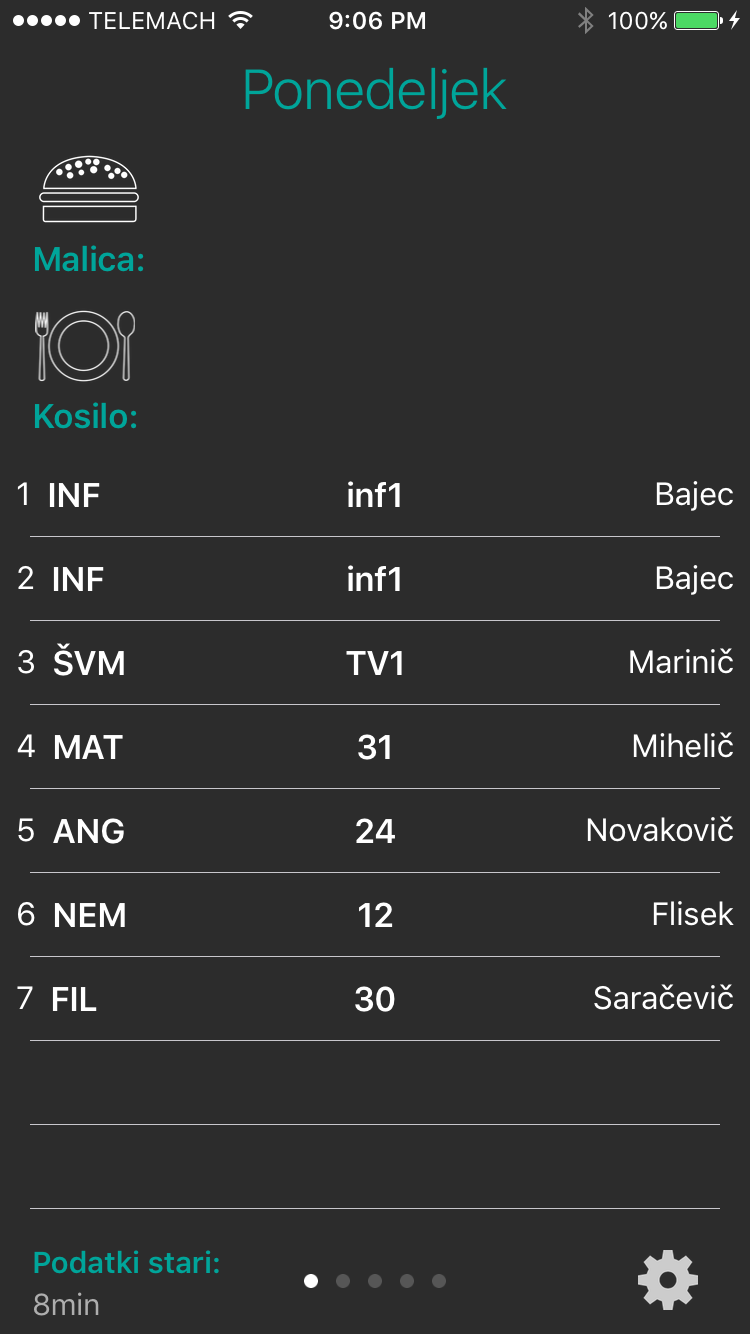
\includegraphics[width=\linewidth]{images/main_view.png}
		\caption{Glavna aktivnost}\label{fig:main_view}
	\end{minipage}\hfill
	\begin{minipage}{0.45\linewidth}
		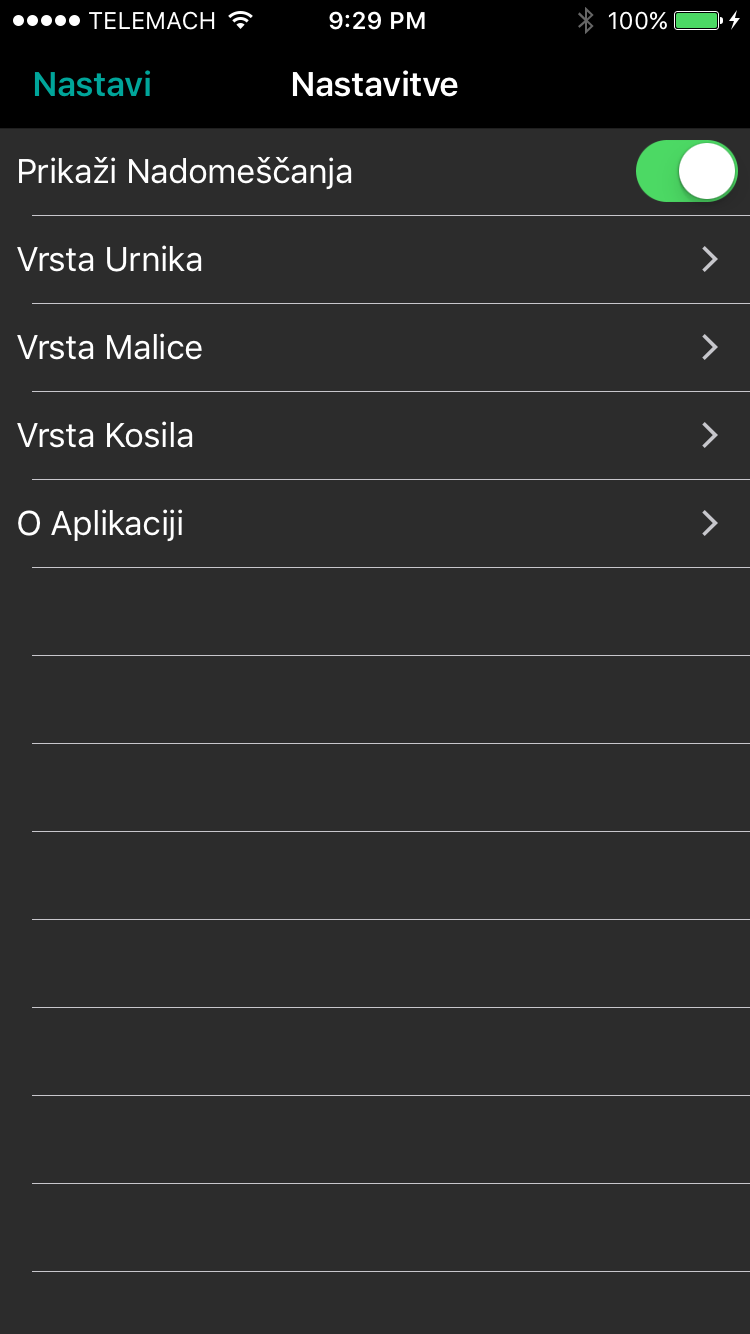
\includegraphics[width=\linewidth]{images/nastavitve.png}
		\caption{Nastavitve}\label{fig:settings}
	\end{minipage}
\end{figure}

\subsubsection{Glavna aktivnost}
\paragraph{}Tu se odvija ve"cino uporabniku pomembnih stvari. Ko uporabnik odpre aplikacijo se mu prika"ze glavni pogled (\textit{ang.} main view) (slika \ref{fig:main_view}) v katerem je za vsak dan prikazan jedilnik in urnik. V glavni aktivnosti se nahaja tudi gumb za nastavitve.

\paragraph{}Ko se aplikacija odpre, najprej preveri, "ce je odprta prvi"c. V tem primeru uporabnika popelje "cez osnovne nastavitve kjer nastavi razred oziroma ime profesorja, ter vrsto malice in kosila. 

\begin{minted}[frame=lines]{swift}
override func viewDidAppear(_ animated: Bool) {
  super.viewDidAppear(animated)

  if UserDefaults().object(forKey:
                           UserSettings.
                           lastRefreshedTimetableData.
                           rawValue) as? Date == nil {
    let setupStoryboard = UIStoryboard(name: "Setup", bundle: nil)
    let viewController = setupStoryboard.instantiateInitialViewController()!
    present(viewController, animated: true, completion: nil)
  }
}
\end{minted}

\paragraph{}
Aplikacija nato prika"ze vse elemente uporabni"ska vmesnika. V osnovi je sestavljen iz \texttt{UIScrollView}-ja, ki skrbi zato, da se lahko premikamo levo in desno. \texttt{UIScrollView} ima ve"c otrok, kjer vsak otrok predstavlja pogled(\texttt{UIView}) za en dan v tednu. Otrok ima eno tekstovno polje (\texttt{UILabel}) v katerem je zapisan dan v tednu in "se dve tekstovni polji v katerih sta zapisana malica in kosilo. Vsak dnevni pogled vsebuje tudi tabelo (\texttt{UITableView}), v kateri je prikazan urnik.

\paragraph{}
V glavni aktivnosti sta prikazana tudi gumb (\texttt{UIButton}) za nastavitve in kako stari so podatki. Starost podatkov nastavimo, ko se aplikacija prika"ze na zaslon. Nato naredimo nov merilnik "casa (\texttt{NSTimer}), ki vsako minuto kli"ce dolo"ceno funkcijo, ki posodobi starost podatkov.

\begin{minted}[frame=lines]{swift}
func setDataAgeLabel() {
  let lastRefreshed = UserDefaults().
                      object(forKey:
                             UserSettings.
                             lastRefreshedTimetableData.
                             rawValue) as? Date
  if lastRefreshed == nil {
    dataAgeLabel.text = "N/A"
  } else {
    let ageText = FuzzyDate.timeSince(lastRefreshed!)
    dataAgeLabel.text = ageText
  }
}
\end{minted}

\subsubsection{Nastavitve}
\paragraph{}V nastavitvah (slika \ref{fig:settings}) lahko uprabnik nastavi ali je dijak, ali profesor in temu primeren filter za urnik. Nastavi lahko tudi vrsto malice in kosila na katerega je naro"cen. Poleg tega ima tudi mo"znost, da izklopi funkcijo za prikaz nadome"s"canj, tako da je uporabniku prikazan samo urnik. V nastavitvah lahko uporabnik pogleda podatke o aplikaciji.

\paragraph{}
Nastavitve se na zaslon prika"zejo kot modalno okno (\texttt{Modal View}). Ko uporabnik zapre nastavitve z pritiskom na gump \textit{Nastavi}, nastavitve sporo"cijo upravitelju podatkov, naj gre po nove podatke.

\begin{center}
	Izhod iz nastavitev:
\end{center}
\begin{minted}[frame=lines]{swift}
@IBAction func doneButtonPressed(_ sender: AnyObject) {
  UserDefaults().synchronize()
  TimetableData.sharedInstance.update()
  navigationController?.dismiss(animated: true, completion: nil)
}
\end{minted}


\subsubsection{O aplikaciji}
\paragraph{}V tem meniju se uporabniku prika"zejo osnovne informacije o aplikaciji kot so avtor aplikacije, verzija in pod katero licenco\cite{license-wiki} je aplikacija izdana. Prav tako je v tem meniju zapisan vir nekaterih ikon, ki so uporabljene, saj to predpisuje licenca pod katero so izdane te ikone.
